\documentclass[12pt,journal,compsoc]{IEEEtran}
\usepackage[margin=1in]{geometry}
\usepackage{graphicx}

\graphicspath{{images/}}



\title{WebStegFS Implementation}
\author{Ryne~Flores, Kyle~Gorak, David~Hart, Matthew~Sjoholm, LTC Timothy Nix \\ \IEEEmembership{Department of Electrical Engineering and Computer Science\\ United States Military Academy}}
\IEEEtitleabstractindextext{
\begin{abstract}
In 2007 Arati Baliga, Joe Kilian, and Liviu Iftode of Rutgers University presented the idea of a web based covert file system~\cite{Baliga2007}. The purpose of a web based covert file system is providing confidentiality and plausible deniability regarding the existence of files. The key components of a web based covert file system is hiding files within media using steganographic techniques using online file sharing for the purpose of collaboration~\cite{Baliga2007}. We implemented such a system, WebStegFS, as a prototype to develop the idea for a web based covert file system previously mentioned. Our prototype of the web based covert file system implements steganographic techniques to obfuscate an entire file system on a public file share site. By storing data in this manner, rather than within the application or on a users computer, we provide confidentiality and plausible deniability to both the users and the companies that manage these public file sharing sites. 
\end{abstract}}
\date{}

\begin{document}
\maketitle

\section{Introduction}

\IEEEPARstart{W}{e} continue to integrate technology more and more in our daily lives because of the convenience it provides to users. Users are becoming connected to the internet in multiple ways nearly everywhere they go. The majority of people interact with multiple forms of technology throughout each day. Some technologies we interact with collect data from our interaction. Also, the widespread use of social media makes it easier to find information about people. Technology, coupled with social media and other applications, can begin to paint a picture used to identify individuals with only non-identifiable information~\cite{VanDam2015}. Sometimes this data collection is used solely to advertise a product to you, but sometimes there are more nefarious means of data collection that lead to black mail, social engineering attacks, or worse. 

The means to store and share information in a covert manner not only serves multiple purposes, but also has various implications depending on how those means are used. There will be innovations designed with the good intentions, yet there will also usually be clever modifications of those designs for malicious intentions. Such examples would include freely expressing and sharing interests ranging from hobbies to religion and sexuality without fear of reprisal or being condemned. However, studies have shown that unethical behavior tends to dominate within the realm of anonymity~\cite{Guitton2013}.

This project is an application that allows users to share information in a covert manner that can provide plausible deniability to not only the users but also to the file sharing or social media site used to store the information. Plausible deniability is ``(The possibility of) denying a fact (especially a discreditable action) without arousing suspicion; the method of achieving this.''\cite{OxfordDictionary} Even if the existence of the file system is uncovered, the data should remain protected and confidential.  

The possibility and threat of cyber attacks on not only individuals but also various infrastructures that are connected to the Internet generates need to securing store information. Encryption is a powerful tool to maintain secrecy of sensitive data and is very important in various institutions such as the financial institution~\cite{Grover2004}. This tool is available to the everyone and will continue to play an important role of information security as not only technology becomes more advanced but also as individuals work to protect their sensitive information from public view on the Internet.

\section{Related Works}

\subsection{StegFS}
There are other projects and systems that have been released which offer users covert methods of sharing information. One such work is StegFS~\cite{Tan2003}.  The concept of StegFS is a designing a file system that contains protected directories which are hidden through the use encryption and steganography. To the extent that these protected directories would not be located or detected unless a password or access key is provided~\cite{Tan2003}. This implementation grants users plausible deniability to the existence of any information contained within those protected directories, yet these protected directories are still stored to an extent within the user's machine. All information used within WebStegFS will only be stored within RAM, thus it increases the security and plausible deniability benefits to users.

In StegFS the hidden files are identified and accessed through their own headers. The encryption is designed to hide the existence of this hidden files from anyone that does not possess the correct access key. StegFS uses the following three data structures to construct the hidden file system: 
\begin{itemize}
\item A link to an inode table that indexes all the data blocks in the file~\cite{Tan2003}
\item A signature that uniquely identifies the file~\cite{Tan2003}
\item A linked list of pointers to free blocks held by the file'~\cite{Tan2003}
\end{itemize}

This file system has been implemented in Linux kernel 2.4 and is available for public download~\cite{Tan2003}. Performance reports have shown that this StegFS implementation was on par with the native Linux file system on a multi-user environment~\cite{2003}.

%\subsection{Tor}

\subsection{CovertFS}
In 2007 three members of the Department of Computer Science from Rutgers' University provided the main concepts and basic outline for the implementation and design of a covert file system\cite{Baliga2007}.  To the best of our knowledge there has been no other implementation of the application described in Rutger's paper, and this project is our take at creating a working prototype which could later be used to develop a successful application or implementation of the covert file system.

CovertFS was a concept of a file system application that would allow users to covertly store and share files on media sharing websites, and where the application could interact with any web based media sharing site~\cite{Baliga2007}. This system was intended to provide complete confidentiality and plausible deniability not only to the users of this application but also to the online media sharing sites that users had covertly stored information on. CovertFS was to accomplish this through the use of advanced Steganography and by not allowing the application to store information on the user's local machine~\cite{Baliga2007}.

%Yet by entering the covert realm of the internet we are allowing our project to criticized on the ethics of it development in accordance with ACM code of Ethics and Professional Conduct\cite{Anderson1993}. Just as Tor is reviewed arguments are brought up against further development\cite{Guitton2013} so to may this project draw vast attention because of what it offers or means to malicious users and intentions.

\section{Design Overview}

In this section, we describe  the architecture of WebStegFS. The five components of WebStegFS that will be described are: the purpose of the web connection in WebStegFS, how the file system is established and operates, how the file system is mapped to photos, the Steganography that WebStegFS uses, and how the file system is encoded.

\subsection{Web Connection}

Our application's interface with the internet needs to serve three purposes:
\begin{enumerate}
\item Retrieve pseudo random images to use for embedding a message. 
\item Upload images to a public online forum anonymously without altering the image.
\item Retrieve specific images from a public online forum anonymously without altering the image. 
\end{enumerate}

After some research, we discovered a service that could satisfy the first purpose. The Cat API provides random cat images retrieved from Tumblr. The API is reliable and returns content neutral images big enough to store information. A downside to this approach is that statistical steganalysis can be done to compare the uploaded images to the originals. The possibility of using local unique images is out of the scope of our project. The next two requirements are fulfilled by Sendspace.com. This website provides an external API that allows our application to easily interface with and upload and download full size images anonymously. 

%The only significant issue that we encountered while using these online resources was with Sendspace.
% At some point, Sendspace updated their API to require a key. We were not aware of this update and our application was completely broken until we found the bug and fixed it.

The online resources work together as follows:
\begin{enumerate}
\item The Cat API retrieves a random cat image for a message to be embedded into.
\item Embed data into image.
\item Upload the encoded image to Sendspace. Sendspace returns and download and delete URL.
\item Download the encoded image using the download URL.
\item Decode the image to restore original data. 
%This allows for the retrieval of the original message. 
\end{enumerate}

\subsection{File System}

The file system in covertFS is built off of the \textit{pyfilesystem} python package, available on the Python Package Index. \textit{Pyfilesystem}, or \textit{fs}, provides a framework of different modules that can access file systems in different locations- one module accesses the running operating system's file system, there is a module for accessing NFS, and finally there is a module that creates and accesses a file system in main memory. This memory-accessing module is called MemoryFS. 

MemoryFS is the superclass for our custom file system class, named (yes, it is the same as the project name) WebStegFS. WebStegFS utilizes CovertFiles (subclassed from MemoryFile) to store the data in files, and CovertEntries (subclassed from MemoryEntry) to store the file metadata (MAC times etc.) of all file system entries, including data files and directories. The WebStegFS class also adds functionality to work alongside the web connection module of the project, such as the URL the corresponding picture can be found at, initial creation time, etcetera. 

In order to mount the user-defined, external, stored-in-memory file system to the native operating system file system, we must use the File system in User Space, or FUSE. FUSE is written in C (to better interact directly with operating system), but there are APIs to use it in other languages--- including Python 3. The python package \textit{fusepy} was our key to accessing FUSE functionality. It provides an easy to use layout for writing a FUSE file system in Python. A FUSE file system is written by defining a function for a list of operations that must be able to be carried out by the operating system--- basically a user definition of how to access each command that can be entered in a command line. Our implementation of this OPERATIONS class is called MemFuse, and it includes a WebStegFS object as a parameter. This allows for dynamic variables to be set by the native operating system (through MemFuse), but then later be accessed by the main function, to upload to the online directory of pictures.

\subsection{Mapping File System Data to Photos}

After the user is done using the file system on their local machine, the data stored within must be uploaded to the online file store. This is done by a three step process.
\begin{enumerate}
\item All data files are uploaded to the online file store, after being processed by the steganography class. The download URL for the uploaded data is stored in the file metadata, in the file system object.
\item The file system is encoded to a string. This includes all directory names, as well as file metadata, such as file names, creation date/time, and the URL at which the file data can be found.
\item The string object that holds all the file system information is sent to the steganography class to be encoded and uploaded. A URL is returned to access the file system at a later time.
\end{enumerate}
Through this process, all information related to the file system is stored in a string, making it available for future use.

%DESIGN OVERVIEW
\subsection{Steganography and CovertFS}
% Section needs additional research
The primary purpose in a web based covert file system is confidentiality and plausible deniability. Using steganography can provide both confidentiality for users as well as plausible deniability. However, steganography also has risks that make it vulnerable to both. Statistical analysis and visible alterations (anything else? -- research) can make steganography detectable, thus removing the aspect of both confidentiality and plausible deniability. However, there are ways to reduce the risks of using steganography. 

\subsubsection{Risks Using Steganography}
%Not enough data

The greatest risk to using steganography, particularly our steganography module, is that an embedded message can be discovered using statistical analysis. Since the original images exist on Tumblr and can be retrieved using the Cat API, our images that get uploaded to Sendspace can be compared to the originals. Statistical analysis between the original and the modified images will indicate that a message has been embeded. There are alternative steganograhpy techniques, but their are still several steganalysis tools to detect them~\cite{Laden}. For example, Virtual Steganography Laboratory (VSL) is a tool developed by Michal Wegrzyn and Pawel Forczmanski, of West Pomeranian University of Technology. VSL has a simple GUI that allows users to select an image and run certain steganalysis modules on that image. The results of the analysis is outputted to an easy-to-read csv file. Figure 1.1 is the original image. Figure 1.2 is the modified image with xxx bytes of data encoded into it. 
%\begin{figure}[h]
%	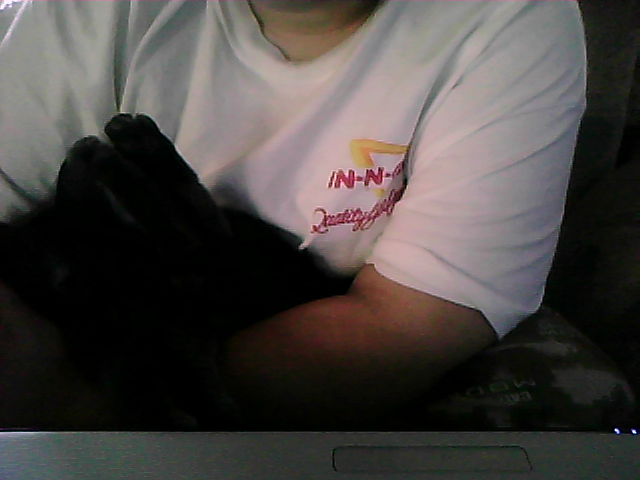
\includegraphics[width=0.5\textwidth]{original}
%	\caption{Figure 1.1. Original image}
%\end{figure}
%\begin{figure}[h]
%	\includegraphics[width=0.5\textwidth]{encoded}
%	\caption{Figure 1.2. Image encoded with a xxx byte message}
%\end{figure}
The VSL determined that there is a message about a xxx byte message in the original image. In reality, there is no message encoded into the original, but this value allows us to compare the two images. VSL determined that the modified image has a xxx byte message encoded into it. ADD VALUES AND FIX ANALYSIS Not only can steganalysis detected changes, but they are visually apparent as well. Figure 1.3 shows both an encoded image and its original.

\begin{figure}[h]
	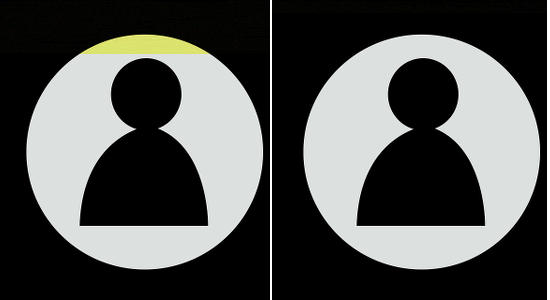
\includegraphics[width=0.5\textwidth]{comparison}
	\caption{Figure 1.3. Left: encoded, Right: original}
\end{figure}
The discoloration at the top of the encoded image is from the LSB encoding and this shows an obvious visual discoloration that an adversary can easily detect.

\subsubsection{Mitigating Risks of Steganography}
%Not enough data
These risks are mitigated by the fact that there is no universal standard for steganography methods. A user can easily replace the steganography module that we offer with a module of their own. That way, even if someone knows an image is not the original, that person will still not know who encoded it, or what kind of module was using for the encoding. Also, an encryption module can easily be added to our application and used to encrypt messages before they are encoded into an image. So even if someone knows what kind of steganography module is being used to encode messages into images, that person will also have the added challenge of decrypting the information. Although, there is no research to indicate that encryption helps in fooling steganalysis tools. Finally, since the original images exist on the internet, it will limit the plausible deniability of the user. It can be called into question as to why a certain user is uploading images that do not belong to that user to an online image database. 

%IMPLEMENTATION SECTION
\subsection{Encoding a File System}

The covert file system uses a drop in steganography module that takes in a bytearray object and returns a URL to an image. We used "least significant bit" steganography for this application because of its simplicity and reliability.

\subsubsection{Steganography Implementation}

Least significant bit (LSB) steganography is a Substitution type of steganography~\cite{Nosrati2011} that replaces the least significant bits in the image's pixels. Our steganography module is not true LSB steganography because we replace multiple bits in each pixel allowing us to encode one byte of data into every pixel. We designed our steganography technique this way to decrease the amount of images required to encode large file systems at the cost of only minimal discoloring. 

First, we break every byte of the message into three segments. Two segments of the byte will contain three bits, and the last segment will contain two bits. Next, we replace the three least significant bits of the red component with the first three bit segment. The green component follows, with the replacement of its least significant bits with the second three bit segment. Lastly, we replace the two least significant bits of the blue component with the remaining two bit segment of data. 

There are obvious drawbacks to our implementation of LSB steganography, primarily that the image may appear distorted as seen in Figure X and CovertFS images are X percent easier to detect using standard statistical analysis techniques compared to true LSB steganography as seen in figure X. However, this implementation enables us to store more bytes than other implementations of LSB steganography which decreases the latency in uploading and downloading images in large file systems [? Need evidence].
 
\subsubsection{File System to Images}

%David, I will need you to describe how the FUSE file system is prepared for encoding. Additionally, I will need information on how the files are uploaded as they are added to the file system (and future parallel upload/download). 
The first step in encoding a file system is retrieving an image. We use "The Cat API" which retrieves a random cat picture from Tumblr or a various number of other sources~\cite{CatAPIDoc}. Once we retrieve the image, we determine the number of bytes we can encode in the image by multiplying the height and width of the image, in pixels. Since we encode one byte per pixel, the result of height times width results in the total number of bytes, \textit{n}, of data we can encode in the image. For example, a 640x480 pixel image can hold 307,200 bytes of data. Next, we take the data we are going to encode and append a special end of file byte encoding. Then, we break the data into two sets, one containing the last \textit{n} bytes and the other the remaining bytes. 

Next, we encode the data in the first set into the image and upload the image. We retrieve the URL of the uploaded image and append a URL identifier byte encoding along with the URL itself to the remaining data. Then, we repeat the encoding steps by appending the end of file byte encoding, splitting the data, and uploading until there is no data left to encode. At this point, we have encoded all the data and have a "linked list" of encoded images containing the data. Finally, we can return the URL to the head image of data. 


\section{Tails}

An implementation that would increase the flexibility and security of this project is developing the WebStegFS into the TAILS operating system and having it run as a bootable program through the a flash drive. The reason for this is because the TAILS operating system in and of itself offers various security measures to ensure a stable and functioning system. We are working to develop a working prototype where our WebStegFS is integrated in the TAILS operating system to further allow confidentality and plausible deniability to the users. 

\section{Future Work}
The current implementation of WebStegFS does not require user authentication to access the file system, it only requires the 6-character code of the file system image to access all files in the system. We use versioning (i.e. the current version of the file system uses this code, if a change is made then a new code will be generated and correspond to the new file system) in order to protect the information stored in the file system from being deleted--- WebStegFS does not ever delete images from the online file storage site, even though some sites allow it. 

An alternative approach could require a user to have an account with the WebStegFS database. This would take away the idea of plausible deniability, as every user would require some sort of entry in the database. However, it could add to the confidentiality of the file system, as only authenticated users would be able to access the data.Another possibility would be to add a simple password entry into the encryption suite. This could increase confidentiality, without removing plausible deniability.

\subsection{Encryption and Advanced Steganography Techniques}

Another future implementation worth looking into is the use of a more advanced steganographic technique. The purpose of this is to ensure the confidentiality and plausible deniability of the users by:
\begin{enumerate}
\item Ensuring that pictures being used to hide the information do not give tell-tale signs of modification
\item To increase the difficulty of steganographic tools discovering the encrypted pictures within the sea of publicly shared images within the file sharing site or social media site that the system it using to store the file system.
\end{enumerate}

There are many different kinds of steganographic techniques that assist in reducing the effectiveness of statistical analysis, recovery of data, and other methods of detection. [?] Other implementations of steganography do not use images at all, but rather encode data within other forms of media such as audio files or PDFs. Using a better steganographic technique in addition to encryption would increase confidentiality and plausible deniability [?]. 

\section{Conclusion}

WebStegFS is the implementation of the CovertFS concept. It is an application that allows users to store and share files covertly through the use of a media sharing site and allows plausible deniability to users and the media sharing sites that they use. It is a modular application that allows users to swap out and customize its various components to include: the type of steganography used, how it establishes a web connection and what media sharing site it uses, and the type of encryption that is used. 

\bibliographystyle{plain}
\bibliography{covertfsrefs}


\end{document}